\documentclass{beamer}
\mode<presentation>
{
  \usetheme{default}     
  \usecolortheme{default}
  \usefonttheme{default}  ...
  \setbeamertemplate{navigation symbols}{}
  \setbeamertemplate{caption}[numbered]
} 

\usepackage[english]{babel}
\usepackage[utf8x]{inputenc}
\usepackage{listings}
\usepackage{amsmath}

\title[Your Short Title]{Gate Problem}
\author{Sanskar Nanegaonkar\\EP18BTECH11016}
\institute{IIT Hyderabad}
\date{February 11, 2020}

\begin{document}

\begin{frame}
  \titlepage
\end{frame}


\begin{frame}{Problem Statement}
\begin{itemize}
    \item EE-2016-Set-1
\end{itemize}

\textit{Question 30:} Consider the following asymptotic Bode magnitude plot ($\omega$ is in rad/s).\\
\vspace{0.4cm}
\begin{figure}
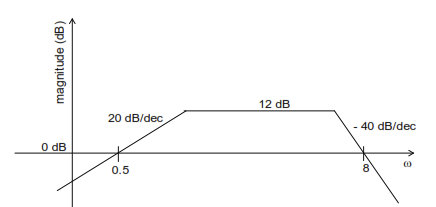
\includegraphics[scale=0.6]{Ques_plot.png}
\caption{Bode Plot}
\end{figure}
\end{frame}

\begin{frame}{}
Which of the following transfer function is best represented by the above Bode magnitude plot?\\
(A) \cfrac{2s}{(1+0.5s)(1+0.25s)^2}\hspace{2cm}
(B) \cfrac{4(1+0.5s)}{s(1+0.25s)}\\
(C) \cfrac{2s}{(1+2s)(1+4s)}\hspace{3cm}
(D) \cfrac{4s}{(1+2s)(1+4s)^2}\\
\end{frame}

\begin{frame}{Solution:}
\begin{itemize}
    \item By looking to the plot, we can say that since the initial slope is +20, there must bea zero at the origin.
    \item Let the corner frequencies of the plot be $\omega_{01}$ and $\omega_{02}$. They can be calculated as follows:
    slope = \cfrac{M_2 - M_1}{log\omega_2 - log\omega_1}\\
    Therefore for $\omega_{02}$,\\
    -40 = \cfrac{0 - 12}{log8 - log\omega_{02}}\\
    log8 - log$\omega_{02}$ = \cfrac{12}{40}\\
    log$\omega_{02}$ = log8 - \cfrac{12}{40}\\
    $\omega_{02}$ = 4\\
\end{itemize}
\end{frame}

\begin{frame}{}
    \begin{itemize}
        \item Therefore for $\omega_{01}$,\\
    20 = \cfrac{0 - 12}{log0.5 - log$\omega_{01}$}\\
    log0.5 - log$\omega_{01}$ = \cfrac{-12}{20}\\
    log$\omega_{01}$ = log0.5 + \cfrac{12}{20}\\
    $\omega_{01}$ = 2
        \item So, the corner frequencies are $\omega_{01}$=2 and $\omega_{02}$ = 4.
        \item At $\omega_{01}$, the change in slope is +20dB, so their exists one pole at this frequency and at $\omega_{02}$, the change in slope is -40dB, so their exists two pole at this frequency.\\
        \item The denominators have the form (1 + \cfrac{s}{\omega})
    \end{itemize}{}
\end{frame}{}

\begin{frame}{}
    \begin{itemize}
        \item So, the denominator of the transfer function is\\ (1 + \cfrac{s}{2})(1 + \cfrac{s}{4})^2\\
        \item Therefore, the transfer function is $\cfrac{sc}{(1 + \cfrac{s}{2})(1 + \cfrac{s}{4})^2}$ where c is some constant\\
        \item The answer is therefore option (A) \cfrac{2s}{(1+0.5s)(1+0.25s)^2}
    \end{itemize}{}
\end{frame}{}

\begin{frame}{Verification}
    \begin{itemize}
        \item We will now plot the bode plot of the given transfer function.
        \item The bode plot is:
            \begin{figure}
            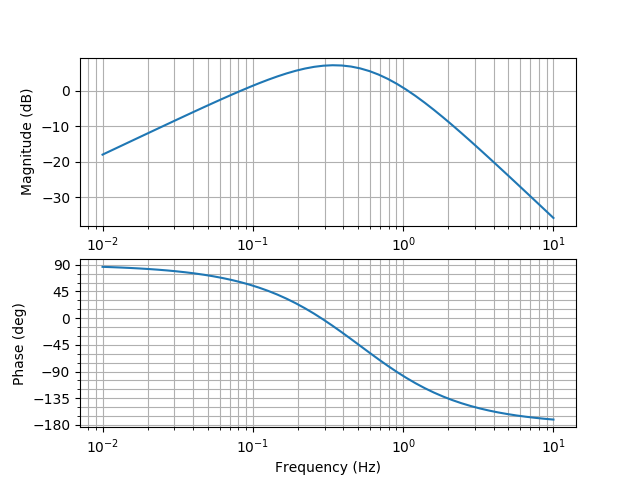
\includegraphics[scale=0.6]{plot.png}
            \caption{Bode Plot}
            \end{figure}
    \end{itemize}{}
\end{frame}{}

\end{document}